\section{Introduction}



%%\subsection{Problem Description}


Developers often use online question and answering (Q\&A) forums,
e.g., StackOverflow (S/O), to learn how to use software libraries and
frameworks. Sometimes, the answer to a question comes as a
fragment/chunk of code, which later makes it to the production
applications, stemming from the copy-and-paste software reuse
practice. Unfortunately, if the copied code fragments are vulnerable,
i.e., possess defects that can potentially be exploited, it will lead
to the applications being prone to attacks. Verdi {\em et
  al.}~\cite{verdi-tse22} reviewed more than 72K C++ code snippets
that migrated from 1,325 S/O answers. Of these, they reported a total
of 99 vulnerable code snippets of 31 different types that made their
way to 2,589 GitHub repositories. Thus, it is crucial to detect early
the vulnerabilities in the code snippets from online forums.
%Running a vulnerability detection tool on the source code after the
%integration of a S/O code snippet into the current codebase would
%waste developers' effort for such integration.

Security researchers have proposed several automated approaches for
vulnerability detection (VD) using program
analysis~\cite{FlawFinder,RATS,viega2000its4,Checkmarx,HPFortify,Coverity,BufferOverFlow,SQLInj,Cross-siteScripting,AuthBypassSpoofing},
as well as machine learning (ML) including deep learning
(DL)~\cite{fse21,chakraborty2020deep,zhou2019devign,li2018sysevr,li2018vuldeepecker}
techniques. However, these approaches warrant the code to exist as
complete program units, often making use of program representations
such~as abstract syntax tree (AST), Program Dependence Graph
(PDG)~\cite{fse21,li2018vuldeepecker}, Control Flow Graph
(CFG)~\cite{zhou2019devign}, Data Flow Graph
(DFG)~\cite{zhou2019devign}, Code Property Graph
(CPG)~\cite{chakraborty2020deep}, etc. At a minimum, they operate at
the method-level granularity, making it impossible to utilize them for
directly detecting vulnerabilities in code snippets. A possible
alternative would be to plug the code snippet into the method, resolve
any ambiguities, and test it with a VD tool. However, such a strategy
is limited. First, if found vulnerable, the efforts of integrating the
code snippet into the existing method would be lost. Second, due to
the black-box
%(inexplicable?)
nature of DL models, we would not know the origin of the
vulnerability, i.e., whether it arises due to the flawed code snippet
or the existing part of the code.

%other statements in the method.

%Besides, even a commit-level VD model requires the code before/after changes to be syntactically valid to extract those features.

Importantly, analyzing code snippets is not straightforward as they
are often incomplete, un-parseable, contain declaration/reference
ambiguity, and are interspersed between user comments. Currently,
there exist tools such as PPA~\cite{ppa08},~which parse an incomplete
code fragment to build the AST and~ex\-tract data types in a
best-effort manner, while StaType \cite{icse18} resolves the libraries
and recovers only the fully-qualified names for references. However,
the basic infrastructure for partial program analysis on incomplete
code snippets is not yet possible. The infrastructure includes the
fundamental supports/services such as lexical, syntactic, and semantic
analysis so that the static and dynamic analysis techniques could be
built upon. Let us call such an infrastructure, {\em partial program
analysis infrastructure}.

In addition to vulnerability detection, such partial program analysis
infrastructure is also beneficial to the other software engineering
(SE) tasks that can tolerate a low level of errors and imprecision in
building the program representations. For example, consider code
completion~\cite{codefill-icse22,facebook-icse21}, in which a model
provides suggestions to complete partial code. Existing ML/DL-based
code completion models are just based on the code sequences or utilize
the syntactic structure in ASTs, but none leverage the program
dependencies due to the nature of partial code. Next, consider the
task of analyzing the code fragments in a bug report to connect it to
the relevant source files for bug localization
purposes~\cite{euler-fse19,icpc17}. Here too, a need for partial
program analysis, especially for partial program dependence analysis,
can be observed.









%\section{Introduction}
Integrating the utilization of program analysis (PA) tools early in the development process of modern, large-scale software systems is crucial in determining the weaknesses/vulnerabilities in the code. Consider, for instance, a scenario in which a developer wants to use an online question and answering (Q\&A) forum, e.g., StackOverflow (S/O), to learn how to use software libraries or frameworks. Typically, the answer to a posed question comes as a fragment/chunk of code, which later makes it to the production application, stemming from the copy-and-paste software reuse practice. Unfortunately, if the copied code fragment is vulnerable, i.e., possesses defects that one can potentially exploit, it will result in the application being prone to attacks. Verdi {\em et al.}~\cite{verdi-tse22} reviewed more than 72K C++ code snippets that migrated from 1,325 S/O answers, reporting a total of 99 vulnerable code snippets of 31 different types that made their way to 2,589 GitHub repositories.

Security researchers have proposed several automated approaches for vulnerability detection (VD) in software systems using program analysis (PA)~\cite{FlawFinder,RATS,viega2000its4,Checkmarx,HPFortify,Coverity}, as well as machine and deep learning (ML \& DL) \cite{fse21,chakraborty2020deep,zhou2019devign,li2018sysevr,li2018vuldeepecker} techniques. These approaches typically leverage program representations such as abstract syntax tree (AST), program dependence graph (PDG)~\cite{fse21,li2018vuldeepecker}, control-flow graph (CFG)~\cite{zhou2019devign}, data-flow graph (DFG)~\cite{zhou2019devign}, code property graph (CPG)~\cite{chakraborty2020deep}, etc., to model the vulnerable features. 
%However, extending such analyses to code snippets is not straightforward as they are often incomplete, unparseable, contain declaration/reference ambiguity, and may be interspersed between user comments. Currently, there exist tools such as PPA~\cite{ppa08}, which parse an incomplete code fragment to build the AST and extract data types in a best-effort manner, while StaType \cite{icse18} resolves the libraries and recovers only the fully-qualified names for references. However, the basic infrastructure for partial program analysis, i.e., for analyzing incomplete code is not yet available. 
%Such an infrastructure must include fundamental supports/services at the structural, semantic, and execution levels, thus enabling the static and dynamic analysis techniques to be built upon. 
%Let us refer to this as \textit{partial program analysis infrastructure}.
However, the PA tools employed to derive these program representations warrant the code to exist as complete program units, at the very least, at the method-level granularity. As a result, it is impossible to utilize such VD tools to find vulnerabilities in code snippets. A possible alternative would be to plug the code snippet into the method, resolve any ambiguities, and test it with a VD tool. However, such a strategy is limited. First, if a vulnerability is found, the efforts of integrating the code snippet into the existing method would be lost. Second, due to the black-box nature of DL models, we would not know the origin of the vulnerability, i.e., whether it arises due to the flawed code snippet or the existing part of the code.

Besides, analyzing code snippets is not straightforward as they are often incomplete, un-parseable, contain declaration/reference ambiguity, and may be interspersed between user comments. Currently, there exist tools such as PPA~\cite{ppa08},~which parse an incomplete code fragment to build the AST and extract data types in a best-effort manner, while StatType \cite{icse18} resolves the libraries and recovers only the fully-qualified names for references. However, the basic infrastructure for partial program analysis, i.e., for analyzing incomplete code is not yet available. Such an infrastructure must include fundamental supports/services at the structural and semantic levels, thus enabling the program analysis techniques to be built upon. Let us refer to this as \textit{partial program analysis infrastructure}.


In addition to vulnerability detection, such an 
%partial program analysis infrastructure 
infrastructure
is also beneficial to other software engineering (SE) tasks that can tolerate a low level of errors and imprecision in building program representations. For example, consider code completion~\cite{codefill-icse22,facebook-icse21}, in which a model provides suggestions to complete partial code. Existing state-of-the-art ML/DL-based code completion models are just based on the code sequences or utilize the syntactic structure in ASTs, but none leverage the program dependencies due to the nature of partial code. Next, consider the task of analyzing the code fragments in a bug report to connect it to the relevant source files for bug localization purposes~\cite{euler-fse19,icpc17}. Here too, a need for partial program analysis, specifically partial program dependence analysis, can be observed.

The other facets of program analysis tools that need to be considered are their soundness and completeness. For example, static analysis tools are designed to detect errors that are valid for all possible executions, which often come at the cost of multiple approximations. As a result, such tools tend to overestimate, resulting in false positives. Next, consider the task of symbolic execution, which is limited by the path explosion problem that hinders its applicability to large-scale software systems. The effectiveness of such a symbolic execution engine can be improved by enhancing the symbolic constraints of the variables, and by guiding it to explore the right subset of symbolic states. 

%While the state-of-the-art research and practice has been well-established for the analysis of the entire programs, very little research and knowledge has been achieved for partial program analysis.

To this effect, we set out to investigate {\tool}, a {\em \underline{Neural} Network-Based \underline{P}rogram \underline{A}nalysis} infrastructure. We aim to establish {\em a scientific foundation, novel methodologies, frameworks, models, and algorithmic solutions for neural program analysis}. We address two major issues in Program Analysis:

(1) {\bf Enabling analysis of incomplete code fragments}, i.e.,
partial program analysis;

(2) {\bf Empowering existing PA tools by making them more sound and
  complete} (Figure~\ref{fig:arch}). {\tool} will allow the
construction of efficient program analysis techniques for (partial)
code on which downstream software engineering applications can be
built.


\subsection{Research Objectives and Anticipated Results}

\begin{figure}[t]
    \centering
    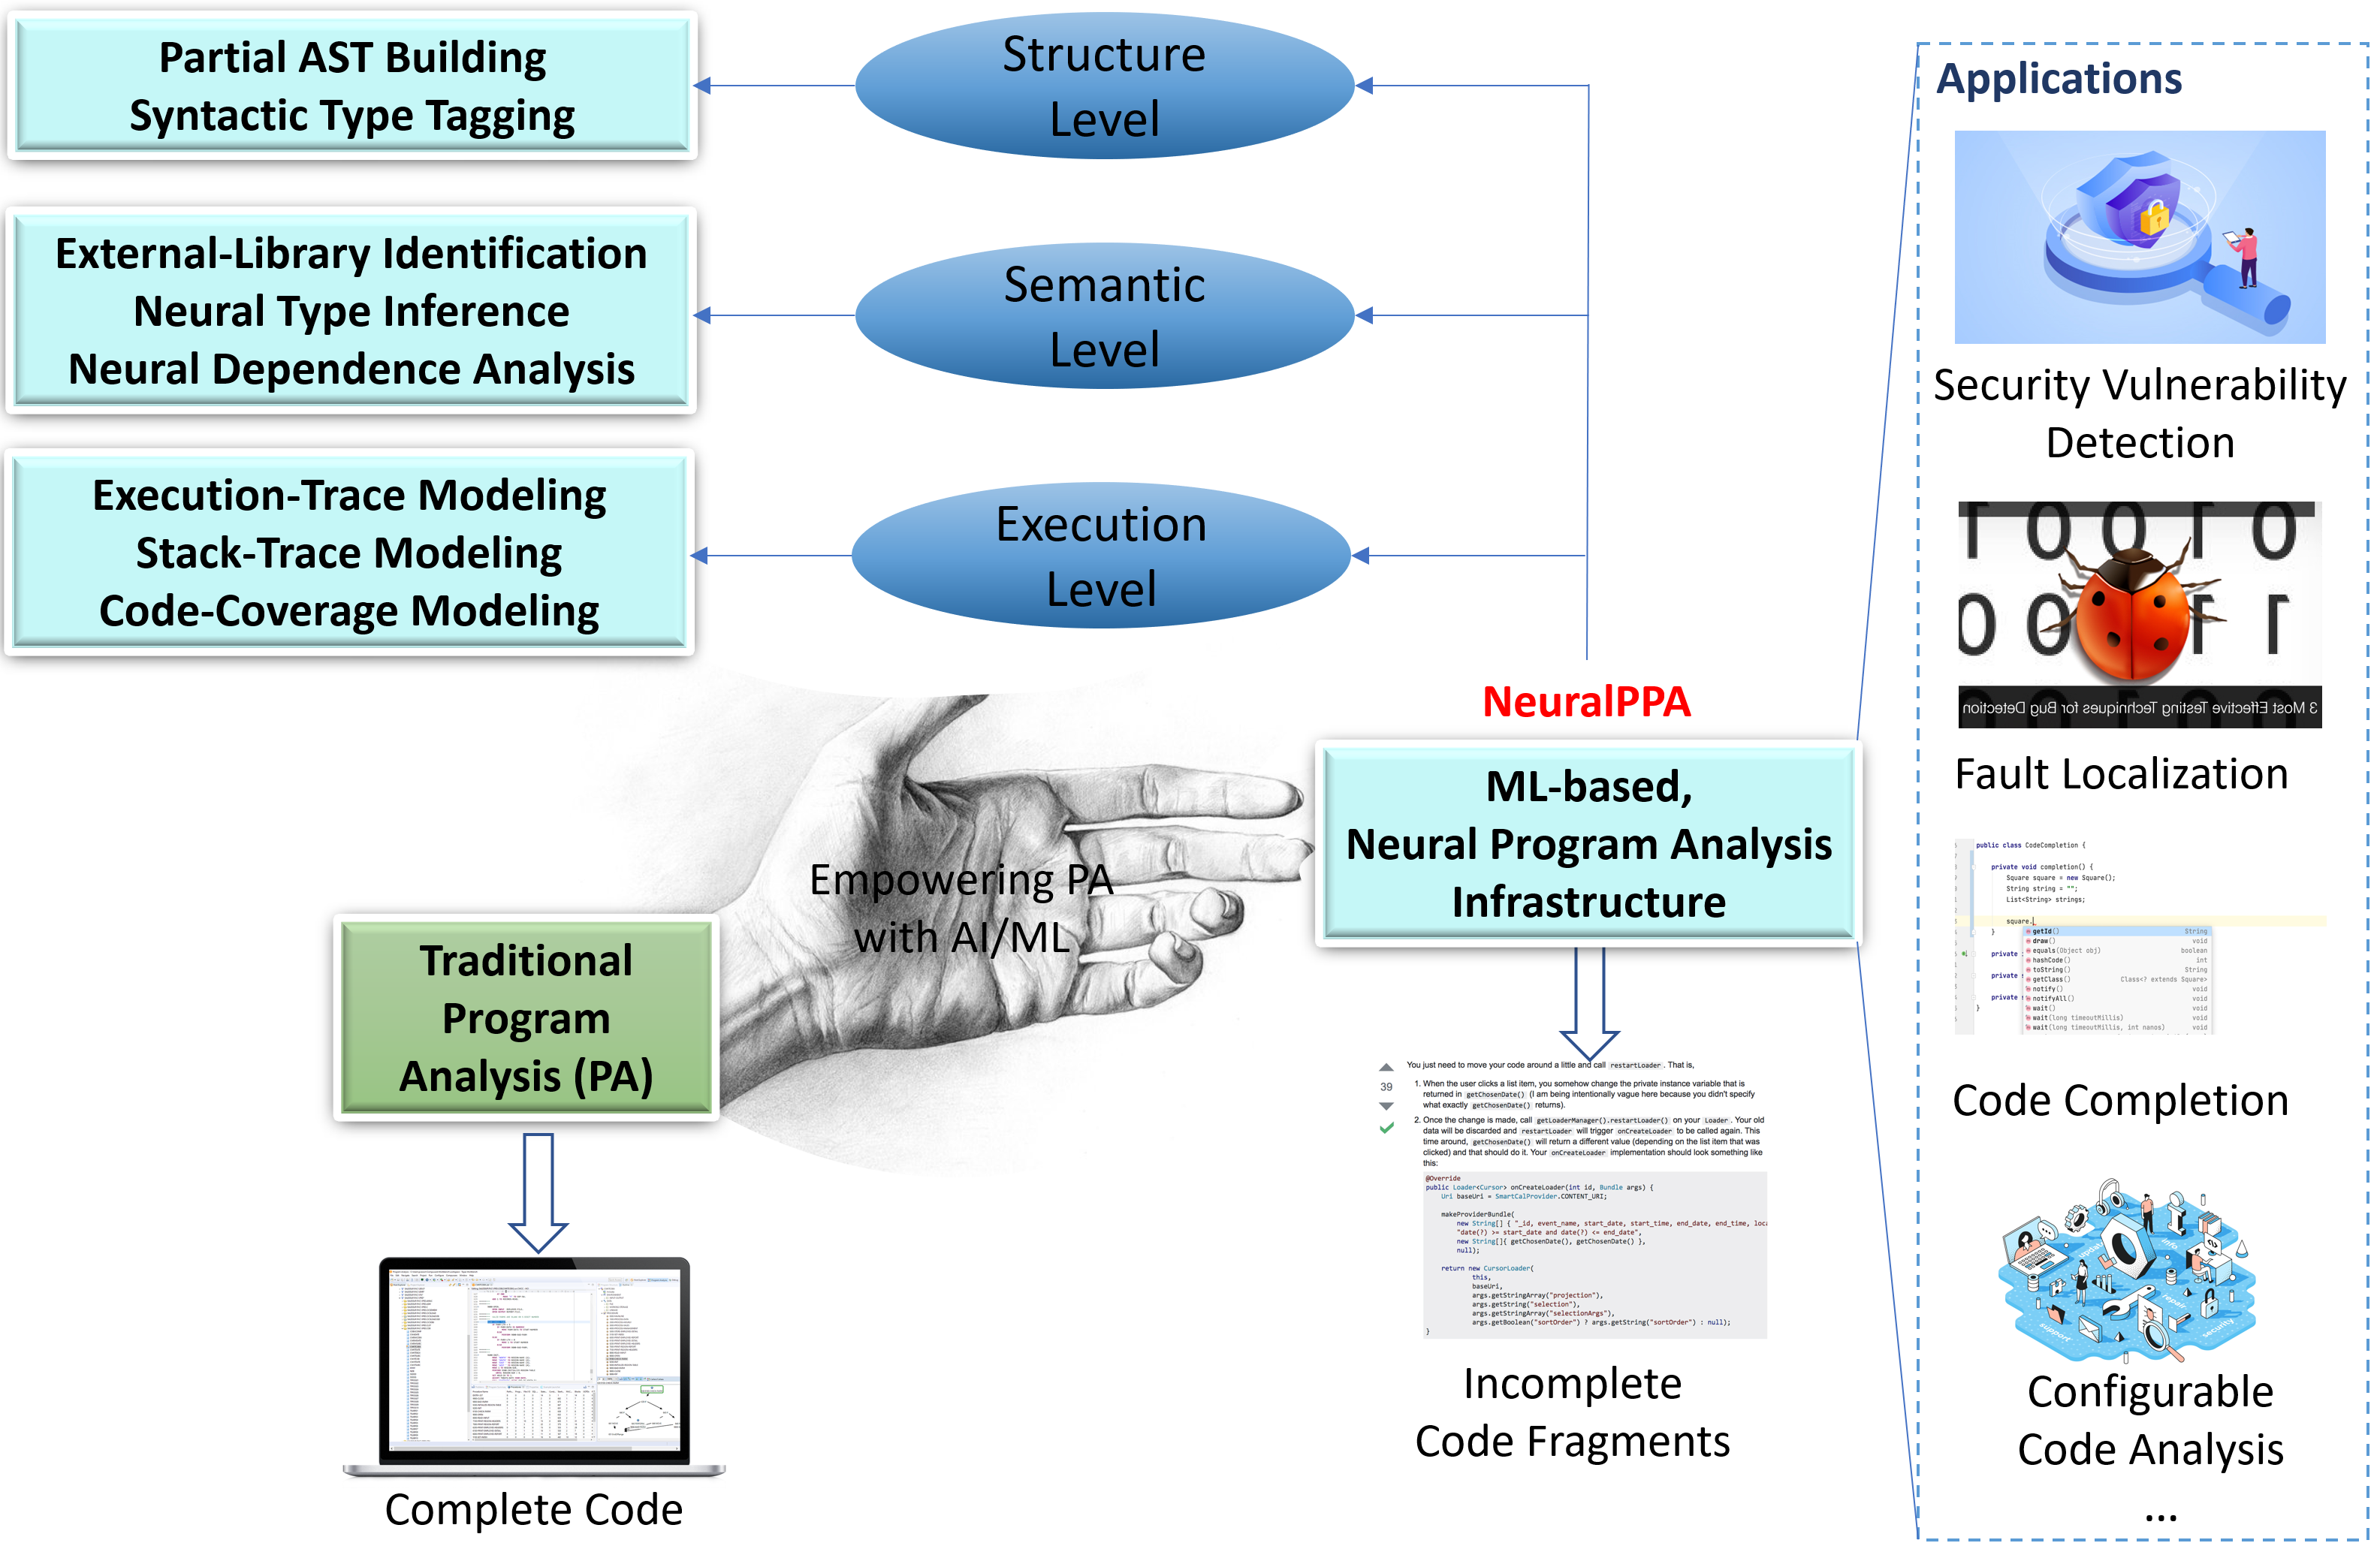
\includegraphics[width=0.9\textwidth]{graphs/neuralppa}
    \vspace{-12pt}
    \caption{{\tool}: Machine Learning-based Program Analysis Infrastructure}
    \label{fig:arch}
\end{figure}


While the state-of-the-art research and practice has been
well-established for the analysis of the entire programs, very little
research and knowledge has been achieved for partial program
analysis.
%
In this proposal, we set out to investigate and develop {\tool}, a
{\em \underline{Neural}-network-based \underline{P}artial
  \underline{P}rogram \underline{A}nalysis infrastructure}. We aim to
develop {\bf a scientific foundation, novel methodologies, frameworks,
  models, and algorithmic solutions for neural partial program
  analysis}. {\tool} {\bf enpowers program analysis (PA) with advanced
machine learning (ML) and artificial intelligence (AI) to enable the
program analysis on incomplete code fragments} (Figure~\ref{fig:arch}).
{\tool} will allow the constructions of the program analysis
techniques for partial code on which downstream software
engineering applications can be built.


In this work, our key philosophy is that {\em the analysis of
  partial code can be learned from the analysis of entire programs in
  the wealth of information from ultra-large-scale, open-source
  software repositories}.



Specifically, we draw our motivation for such a data-driven,
learning-based approach from the following. First, ultra-large-scale
software repositories, e.g. GitHub (7M+ projects) and SourceForge
(700k+ projects) contain an enormous collection of programs. These
repositories amount to 1,000,000,000+ lines of code, 10,000,000+
revision logs, and 3,000,000+ issue reports. This wealth of knowledge
is an excellent source for {\tool}. Hindle {\em et
  al.}~\cite{naturalness-icse12} have shown that code has high
repetitiveness and predictability, and can be captured well by
statistical models. Thus, we expect to build ML models to learn from
those repositories. Second, in an empirical study on the
repetitiveness, containment, and composability of PDGs in open-source
projects, the PI group~\cite{msr16} reported that among
17.5M PDGs with 1.6B PDG subgraphs, 14.3\% of the PDGs have all of
their subgraphs repeated across different projects. Furthermore, in
15.6\% of the PDGs, at least 90\% of their subgraphs are likely to
have appeared before in other projects. Thus, {\tool} could learn from
PDGs with complete program dependencies retrieved from existing code
repositories and derive the dependencies for the (partial) code
fragment under study. The PI group also reported a high repetitiveness
level for AST code structure in open-source
projects~\cite{icse15}. Finally, such a program analysis
infrastructure like {\tool} can be drawn from the spirit and successes
of the approaches in natural language processing (NLP). For example,
at the lexical level, the task of deriving the token types for source
code tokens could be analogous to the part-of-speech (PoS) tagging in
NLP. At the syntax level, the task of learning the syntactic structure
in AST of the partial code can be inspired by the approaches to build
parse trees for natural-language texts. At the semantic level, the
partial program dependence analysis infrastructure is similar in
spirit to the the neural network-based dependency parsing in NLP,
which learns the dependencies signifying the semantic relationships
between words in a sentence from text corpora.

Toward this theme, in our preliminary work, we developed DeepPDA, a neural
network-based partial program dependence analysis approach that learns
to derive the program dependencies for any code fragments (i.e., both
complete and incomplete). In our preliminary empirical evaluation, we
intrinsically evaluated it on Java and C/C++ programs. First, we
trained {\tool} on complete code. For testing, we treated each method
individually and chose a consecutive portion within the method to
predict the program dependencies, and compared them against the actual
dependencies. Overall, DeepPDA predicts CFG and PDG edges in Java
with an F-score of 94.29\%, and in C++ with an F-score of
92.46\%.
%
We also developed as an approach to derive the data
types of the variables in the code snippets. We treat the problem as
statistical machine translation from source code with partially
qualified names to source code with FQNs of the APIs. Our empirical
evaluation on real-world code and StackOverflow posts shows that our
technique achieves high accuracy with 97.6\% precision and 96.7\%
recall in deriving data types in code snippets.


In {\tool}, we propose the following thrusts of research
(Table~\ref{tab:milestones}):

\vspace{3pt}
\noindent \textbf{Thurst 1. Neural Structural Analysis Infrastructure
  \code{NeuralStruct}.} ({\em Section~\ref{}}) Source code has
well-defined structures and semantics. Thus, the basic infrastructure
in {\tool} is the neural structural analysis (\code{NeuralStruct})
component.  This component has two main tasks. First, it learns from
the syntactic structures of the complete code in the training dataset
collected from large-scale code repositories, to derive the abstract
syntax tree (AST) that best represents the syntactic structure of the
given partial code, i.e., with the highest likelihood/probability.
The traditional lexical analyzer still works for partial code due to
the independence nature of lexical tokens. The second task of this
component is to tag the code tokens with the types of the syntactic
units including the statement types (\code{if}, \code{for}, etc.),
variables, fields, methods, classes, etc. Both of the tasks can be
performed with our learning-based approaches in a dual-learning
manner.
  
\vspace{3pt}
\noindent \textbf{Thurst 2. Neural Semantic Analysis Infrastructure.}
({\em Section~\ref{}}) The basis components for several program
analysis techniques include the following:

1) the identification of the APIs of the external libraries in the
external references in the partial code: this is needed because the
partial code contains the undeclared reference and/or
declaration/reference ambiguity without explicit declaration of the
APIs in the external libraries.

2) the inference of the type information for the entities in the
partial code: due to the ambiguity in the declaration, the types of
the variables and statements are not always obviously defined. Thus,
the type inference is a basic service within {\tool}.

3) the inference of the program dependencies among the statements in
the partial code: several program analysis techniques are based on the
program dependencies, which are not always obtainable due to the
incompleteness of the given code fragment.

\vspace{3pt}
\noindent \textbf{Thurst 3. Neural Symbolic Execution Infrastructure.}
...

\vspace{3pt}
\noindent \textbf{Thurst 4. Neural Partial Program Analysis
  Applications.}  ({\em Section~\ref{}}) Our last thrust of research
is aimed to evaluate our basic partial program analysis infrastructure
in a few applications. We choose the following software engineering
applications: 1) software vulnerability detection for code snippets,
2) fault localization, and 3) code completion.

\vspace{3pt}
\noindent \textbf{Thurst ???. Neural Execution Analysis Infrastructure.}
({\em Section~\ref{}}) All the dynamic analysis techniques require the
analysis and understanding of the execution. However, for an
incomplete code, we first need to design a component that can wrap
around the given code fragment with the minimum code so that the code
fragment can be executed. When the code is executed, we also need the
approaches that represent the executed statements and their relations,
model the execution and stack traces, and model the code coverages
for an execution.


\begin{table*}[t]
	\vspace{-15pt}
\begin{center}
{\footnotesize{
\begin{tabular}{cc}
\begin{tabular}[t]{|p{0.2in}|p{2.95in}|} 
\hline
\multicolumn{2}{|>{\columncolor[gray]{0}}c|}{\textcolor{white}
{\bf Year 1 Project Milestones \& Deliverables}}\\
\hline 
\hline
\multicolumn{2}{|c|}{\bf T1. Neural Structure Analysis Infrastructure}\\
\hline
{\bf 1.1} & Neural Syntactic Type Tagging\\
{\bf 1.2} & Neural Partial AST Building\\
{\bf 1.3} & Evaluation of the components\\
\hline
\hline
\multicolumn{2}{|c|}{\bf T2. Neural Semantic Analysis Infrastructure}\\ 
\hline
{\bf 2.1} & External-Library Identification\\
\hline
%\hline
%\multicolumn{2}{|c|}{\bf Integrate Code Synthesis into Tools}\\
%\hline
%{\bf 1.5} & \goalOneFour.\\
%\hline
\multicolumn{2}{c}{}
\end{tabular}
&
\begin{tabular}[t]{|p{0.2in}|p{2.95in}|} \hline
\multicolumn{2}{|>{\columncolor[gray]{0}}c|}{\textcolor{white}
{\bf Year 2 Project Milestones \& Deliverables}}\\
\hline 
\hline
\multicolumn{2}{|c|}{\bf T2. Neural Semantic Analysis Infrastructure}\\
\hline
{\bf 2.2} & Neural Type Inference\\
{\bf 2.3} & Neural Dependence Analysis\\
%{\bf 2.3} & Integrate Evaluation Framework into Design Environment\\
%{\bf 2.4} & Evaluate CRL Framework with Existing Models\\
%{\bf 2.3} & \goalTwoThree.\\

\hline
\hline
\multicolumn{2}{|c|}{\bf T3. Neural Execution Analysis}\\ 
\hline
%{\bf 3.1} & Design New Code Representations and Learning Models.\\
{\bf 3.1} & Neural Execution-Trace Modeling\\
%{\bf 2.4} & Advance FL and RT-CI Approaches.\\
%{\bf 2.5} & Advance Regression Testing in CI Approaches.\\
%{\bf 2.5} & Advance APR Approaches with Framework.\\
\hline
%\hline
%\multicolumn{2}{|c|}{\bf Community Involvement: Capacity Building}\\
%\hline
%{\bf 2.4} & \goalTwoFour.\\
%{\bf 2.5} & \goalTwoFive.\\
%{\bf 2.6} & \goalTwoSix.\\
%\hline
\multicolumn{2}{c}{}
\end{tabular}
\end{tabular}\\
\vspace*{-.3cm}
\begin{tabular}{c}\hline
\multicolumn{1}{|>{\centering\columncolor[gray]{0}}p{6.44in}|}{\textcolor{white}
{\bf Year 3 Project Milestones \& Deliverables}}\\
\hline
\end{tabular}\\
\vspace*{-.2cm}
\begin{tabular}{cc}
\begin{tabular}[t]{|p{0.2in}|p{2.95in}|}
\hline
\multicolumn{2}{|c|}{\bf T3. Neural Execution Analysis}\\
\hline
{\bf 3.2} & Neural Stack Trace Modeling\\
{\bf 3.3} & Neural Code Coverage Modeling\\

%{\bf 3.3} & Testing on Models in IDE tools.\\
\hline
%\hline
%\multicolumn{2}{|c|}{\bf \goalTwo}\\ 
%\hline
%{\bf 3.3} & \goalThreeThree.\\
%\hline
\multicolumn{2}{c}{}
\end{tabular}
&
\begin{tabular}[t]{|p{0.2in}|p{2.95in}|}
\hline
\multicolumn{2}{|c|}{\bf T4. Neural Partial Program Analysis Applications}\\
\hline
%{\bf 3.1} & Design New Code Representations\\

{\bf 4.1} & Security Vulnerablity Detection with {\tool}\\
{\bf 4.2} & Fault Localization and Completion with {\tool}\\

\hline
\multicolumn{2}{c}{}
\end{tabular}
\end{tabular}
\vspace{-15pt}
}}
\end{center}
\vspace*{-.3in}
%\caption{Tasks and Milestones. (Rep. = Representation)}
\caption{The 3-year schedule of Thrusts, Tasks, and Milestones of this proposal.}
%the schedule of Thrusts, Tasks, and Milestones of this proposal.
%\vspace{-10pt}
\label{tab:milestones}
\vspace{-10pt}
\end{table*}
%






%\subsection{Significance of This Proposed Project: NSF Merit Criteria}

\section{Intellectual Merits}

The results of this project will advance the state-of-the-art
knowledge and scientific foundations in both program analysis and
machine learning. They are transformative and directly help improve
software quality with novel program analysis and vulnerability
detection tools.

\noindent \underline{{\bf Advance the state-of-the-art knowledge and
    understanding}}. Neural program analysis infrastructure in Thrusts
1--3 will advance the body of knowledge and theoretical foundations
for machine learning and AI for code. Thrust 4 will help advance the
practical tools for software security and engineering.

\noindent \underline{{\bf Scientific foundation, creative/original
    research}}. This project will provide a scientific
foundation (novel concepts, representations, algorithms, models,
and tools) (1) to enable the analysis on partial code, (2) to empower
the program analysis techniques on both (in)complete code,
and (3) to enable the applications of program analysis on incomplete
code such as vulnerability detection on code snippets, code
completion, etc.

\section{Broader Impacts}

\underline{{\bf (1) Transformative and benefits to society}}. Our
results will be transformative and directly benefit to our society.
They will lead to increasing developers' productivity, software
quality \& reliability.  Our validation involves students and
professionals, promoting teaching, training, and learning of both {\bf
  program analysis} and {\bf machine learning} techniques that
have wide impacts in industry and academic communities.

\noindent\underline{{\bf (2) Foster other related research
    activities}}. Our results will foster {\em research activities in
  related fields of {\bf deep learning} and {\bf software
    security}}. This project will produce theoretical concepts and
techniques that are novel even in deep learning, e.g., novel neural
networks to model and learn for code. The applications of our neural
program analysis in software engineering applications will advance
software security and reliability.

%The collected {\bf large scale bug\&fix corpus} will be useful for
%software quality and reliability research.
%Innovations in CRL could be used to {\bf advance other SE tasks}. We
%will also develop {\bf novel DL-based bug detect-fix} approaches.


\noindent\underline{{\bf (3) Education, dissemination, and broader participation}} (Section~\ref{edu}). The
research will enhance the infrastructure for teaching/research via
tools and data sets for use by students and practitioners, and for
enhancement by researchers. We will provide related learning
modules for educators as well. It will include outreach activities for
undergraduate students, underrepresented groups, minorities, and women
in science.
%contribute novel
%teaching modules to our curriculum.
%Details will be presented in Section~\ref{edu}


\iffalse
\begin{itemize}
	\vspace{-5pt}
\itemsep-0.2em 
  \item {\bf Transformative and benefits to society}. Our 
    results will be transformative and directly benefit to our
    society. 
    They will lead to increasing developers' productivity
    and software quality \& reliability. 
    Our validation involves students and
    professionals, promoting teaching, training, and learning of bug detecting and fixing techniques that have wide impacts 
    in industry and academic communities.

%report

  \item {\bf Foster other research activities}. Our results will
    foster research activities in related fields of deep learning and
    software quality. 
    This project will produce theoretical
    concepts and techniques that are novel even in deep learning, e.g.,
    novel neural networks for modeling and learning code. 
    The collected large scale bug fixing corpus will be useful for software quality and reliability research in general.
    %e.g.,   code transformation. 
%    This project will also advance
%    the state-of-the-art research in large-scale program analysis with
%    deep neural network models.

%The representation for software security vulnerabili will be useful in
%research on software security, malware detection, vulnerability
%reports, and automatic security patching.


  \item {\bf Education, dissemination, and broader participation}.
  The research will enhance the infrastructure for teaching and
  research by providing tools and data sets for use by students and
  practitioners, and for enhancement by other researchers. We will
  provide related learning modules for educators as well. It will
  contribute novel teaching modules to our curriculum. Details will be
  presented in Section~\ref{edu}

%Details are in Section 4.

\end{itemize}
\fi
